% Homecastr Investor Pitch Deck - V4 Honest Competitive Positioning
% Compile with: xelatex homecastr_pitch_v4.tex

\documentclass[aspectratio=169,12pt]{beamer}

% ─── Theme & Colors ──────────────────────────────────────────
\usetheme{default}
\usecolortheme{default}
\setbeamertemplate{navigation symbols}{}
\setbeamertemplate{footline}{%
  \ifnum\thepage>1\relax%
    \hbox to \paperwidth{%
      \kern1em{\scriptsize\href{https://homecastr.com}{\textcolor{hcGold}{Homecastr}}}%
      \hfill%
      {\usebeamercolor[fg]{page number in head/foot}\usebeamerfont{page number in head/foot}\insertframenumber}%
      \kern1em%
    }\vskip2pt%
  \fi%
}
\setbeamertemplate{frametitle}{
  \vspace{10pt}
  \begin{beamercolorbox}[wd=\paperwidth,center]{frametitle}
    \usebeamerfont{frametitle}\insertframetitle
    \par\vspace{4pt}
    {\color{hcGold}\hrule height 1.5pt width 4cm}
  \end{beamercolorbox}
}

% Homecastr brand palette
\definecolor{hcBg}{HTML}{F2EDE0}
\definecolor{hcText}{HTML}{3D3830}
\definecolor{hcGold}{HTML}{CA8A04}
\definecolor{hcGoldLight}{HTML}{E8D5A0}
\definecolor{hcMuted}{HTML}{7E7B74}
\definecolor{hcCard}{HTML}{EBE4D6}
\definecolor{hcRed}{HTML}{B91C1C}
\definecolor{hcGreen}{HTML}{15803D}

\setbeamercolor{background canvas}{bg=hcBg}
\setbeamercolor{normal text}{fg=hcText}
\setbeamercolor{frametitle}{fg=hcText}
\setbeamercolor{title}{fg=hcText}
\setbeamercolor{subtitle}{fg=hcMuted}
\setbeamercolor{itemize item}{fg=hcGold}
\setbeamercolor{itemize subitem}{fg=hcGold}
\setbeamertemplate{itemize item}{\raisebox{1pt}{\tikz{\node[regular polygon, regular polygon sides=6, fill=hcGold, inner sep=0pt, minimum size=3.5pt] {};}}}
\setbeamertemplate{itemize subitem}{\raisebox{1pt}{\tikz{\node[regular polygon, regular polygon sides=6, fill=hcGold, inner sep=0pt, minimum size=2.5pt] {};}}}


\setbeamerfont{title}{size=\Huge,series=\bfseries}
\setbeamerfont{frametitle}{size=\Large,series=\bfseries}
\setbeamerfont{subtitle}{size=\large}

% Packages
\usepackage{fontspec}
\setmainfont{Segoe UI}
\setsansfont{Segoe UI}
\usepackage{tikz}
\usetikzlibrary{calc,positioning,arrows.meta,shapes.geometric}
\usepackage{graphicx}
\usepackage{booktabs}
\usepackage{hyperref}

% ─── Macros ──────────────────────────────────────────────────
\newcommand{\goldtext}[1]{{\color{hcGold}#1}}
\newcommand{\mutedtext}[1]{{\color{hcMuted}#1}}
\newcommand{\statbox}[2]{%
  \begin{minipage}[t]{0.22\textwidth}
    \centering
    {\Huge\bfseries\color{hcGold}#1}\\[4pt]
    {\small\color{hcMuted}#2}
  \end{minipage}%
}

% Logo image macro
\newcommand{\buildingicon}{%
\includegraphics[height=1.2cm]{homecastr-logo.png}%
}

% Big stat macro for single-stat visual slides
\newcommand{\bigstat}[2]{%
  {\fontsize{64}{72}\selectfont\bfseries\color{hcGold}#1}\\[8pt]
  {\Large\color{hcText}#2}%
}

% ══════════════════════════════════════════════════════════════
\begin{document}

% ─── SLIDE 1: Title ──────────────────────────────────────────
\usebackgroundtemplate{\includegraphics[width=\paperwidth,height=\paperheight]{title_bg.png}}
\begin{frame}[plain]
\vfill
\begin{center}
{\buildingicon}\quad{\fontsize{42}{48}\selectfont\bfseries\color{hcGold} Homecastr}\\[16pt]
{\Large\color{hcText} The foundation model for residential real estate}\\[24pt]
\mutedtext{\small \href{https://homecastr.com}{\textcolor{hcGold}{\textbf{homecastr.com}}}}
\end{center}
\vfill
\end{frame}

% ─── Default background for remaining slides ─────────────────
\usebackgroundtemplate{%
  \begin{tikzpicture}[remember picture,overlay]
    \fill[hcBg] (current page.south west) rectangle (current page.north east);
  \end{tikzpicture}
}


% ─── SLIDE 2: The Gap ────────────────────────────────────────
\begin{frame}{Everyone Knows What a Home Is Worth Today}
\vspace{4pt}

\begin{center}
{\large\color{hcText} Nobody can affordably show you where it's \goldtext{going}.}
\end{center}

\vspace{12pt}

\begin{columns}[c]
\begin{column}{0.44\textwidth}
\begin{center}
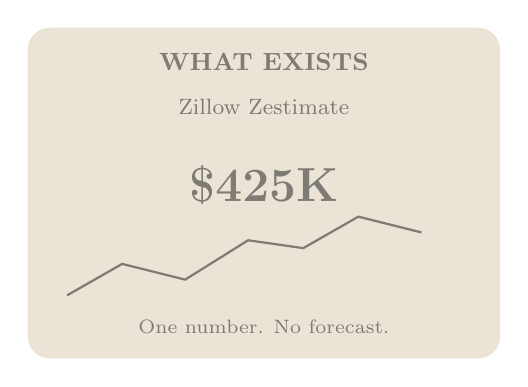
\begin{tikzpicture}
  % "Today" box — static point estimate
  \fill[hcCard, rounded corners=8pt] (0,0) rectangle (6.0,4.2);
  \node[anchor=north, font=\small\bfseries, text=hcMuted] at (3.0,4.0) {WHAT EXISTS};
  \draw[hcMuted, thick] (0.5,0.8) -- (1.2,1.2) -- (2.0,1.0) -- (2.8,1.5) -- (3.5,1.4) -- (4.2,1.8) -- (5.0,1.6);
  \node[font=\footnotesize, text=hcMuted, align=center] at (3.0,3.2) {Zillow Zestimate};
  \node[font=\LARGE\bfseries, text=hcMuted] at (3.0,2.2) {\$425K};
  \node[font=\scriptsize, text=hcMuted] at (3.0,0.4) {One number. No forecast.};
\end{tikzpicture}
\end{center}
\end{column}
\begin{column}{0.08\textwidth}
\begin{center}
{\fontsize{28}{32}\selectfont\color{hcGold}\textbf{→}}
\end{center}
\end{column}
\begin{column}{0.44\textwidth}
\begin{center}
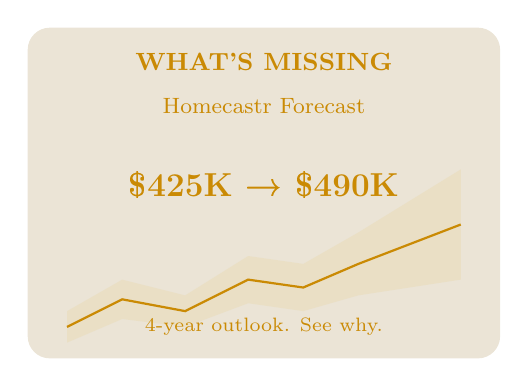
\begin{tikzpicture}
  % "Tomorrow" box — forecast bands
  \fill[hcCard, rounded corners=8pt] (0,0) rectangle (6.0,4.2);
  \node[anchor=north, font=\small\bfseries, text=hcGold] at (3.0,4.0) {WHAT'S MISSING};
  % Forecast band fill
  \fill[hcGoldLight, opacity=0.3] (0.5,0.6) -- (1.2,1.0) -- (2.0,0.8) -- (2.8,1.3) -- (3.5,1.2) -- (4.2,1.6) -- (5.5,2.4)
    -- (5.5,1.0) -- (4.2,0.8) -- (3.5,0.6) -- (2.8,0.7) -- (2.0,0.4) -- (1.2,0.5) -- (0.5,0.2) -- cycle;
  % Median forecast line
  \draw[hcGold, thick] (0.5,0.4) -- (1.2,0.75) -- (2.0,0.6) -- (2.8,1.0) -- (3.5,0.9) -- (4.2,1.2) -- (5.5,1.7);
  \node[font=\footnotesize, text=hcGold, align=center] at (3.0,3.2) {Homecastr Forecast};
  \node[font=\large\bfseries, text=hcGold] at (3.0,2.2) {\$425K → \$490K};
  \node[font=\scriptsize, text=hcGold] at (3.0,0.4) {4-year outlook. See why.};
\end{tikzpicture}
\end{center}
\end{column}
\end{columns}

\vspace{8pt}
\begin{center}
\mutedtext{\small 150M+ residential properties. Forecasts exist --- but none built for consumers.}
\end{center}
\end{frame}


% ─── SLIDE 3: Live Product ───────────────────────────────────
\begin{frame}{See It Live}
\vspace{4pt}

\begin{center}
{\large See where any property is heading, not just where it's been.}
\end{center}

\vspace{8pt}

\begin{columns}[c]
\begin{column}{0.33\textwidth}
\centering
\includegraphics[width=4cm]{scenarios.png}\\[4pt]
{\footnotesize\goldtext{Scenario Analysis}}\\
{\scriptsize\mutedtext{What-if modeling}}
\end{column}
\begin{column}{0.33\textwidth}
\centering
\includegraphics[width=4cm]{pricebands.png}\\[4pt]
{\footnotesize\goldtext{Forecast Bands}}\\
{\scriptsize\mutedtext{Not a point estimate}}
\end{column}
\begin{column}{0.33\textwidth}
\centering
\includegraphics[width=4cm]{explainable.png}\\[4pt]
{\footnotesize\goldtext{Explainable Outputs}}\\
{\scriptsize\mutedtext{For investment memos}}
\end{column}
\end{columns}

\vspace{12pt}
\begin{center}
\mutedtext{\small \href{https://homecastr.com}{\textcolor{hcGold}{\textbf{homecastr.com}}} \quad Free. Live. Interactive.}
\end{center}
\end{frame}


% ─── SLIDE 4: How It Works ───────────────────────────────────
\begin{frame}{How It Works}
\vspace{16pt}

\begin{center}
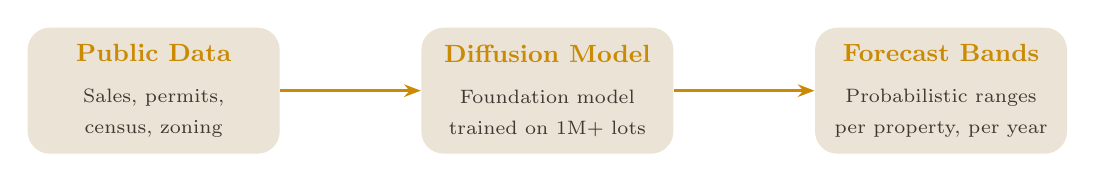
\begin{tikzpicture}[
  block/.style={rounded corners=8pt, fill=hcCard, text=hcText,
    minimum width=3.2cm, minimum height=1.6cm, align=center, font=\small},
  arr/.style={-{Stealth[length=6pt]}, very thick, color=hcGold}
]
  \node[block] (data) at (0,0) {
    \goldtext{\textbf{Public Data}}\\[4pt]
    {\scriptsize Sales, permits,}\\
    {\scriptsize census, zoning}
  };
  \node[block] (model) at (5,0) {
    \goldtext{\textbf{Diffusion Model}}\\[4pt]
    {\scriptsize Foundation model}\\
    {\scriptsize trained on 1M+ lots}
  };
  \node[block] (output) at (10,0) {
    \goldtext{\textbf{Forecast Bands}}\\[4pt]
    {\scriptsize Probabilistic ranges}\\
    {\scriptsize per property, per year}
  };

  \draw[arr] (data) -- (model);
  \draw[arr] (model) -- (output);
\end{tikzpicture}
\end{center}

\vspace{20pt}

\begin{center}
\statbox{14\%}{Median Error}
\hfill
\statbox{4yr}{Forecast Horizon}
\hfill
\statbox{1M+}{Properties Indexed}
\hfill
\statbox{<1s}{API Response}
\end{center}
\end{frame}


% ─── SLIDE 5: Why Now ────────────────────────────────────────
\begin{frame}{Why Now}
\vspace{16pt}

\begin{columns}[c]
\begin{column}{0.48\textwidth}
\begin{center}
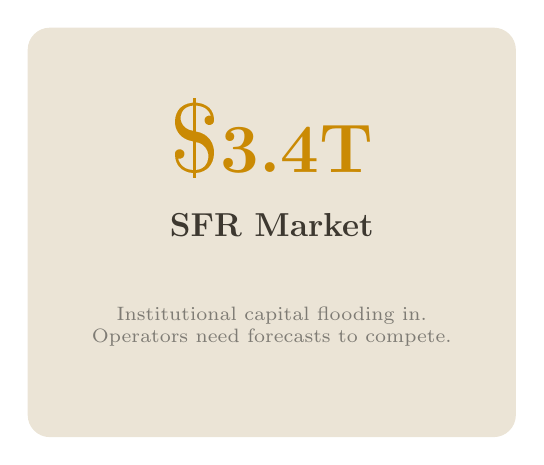
\begin{tikzpicture}
  \fill[hcCard, rounded corners=8pt] (0,0) rectangle (6.2,5.2);
  \node[font=\fontsize{40}{46}\selectfont\bfseries, text=hcGold] at (3.1,3.8) {\$3.4T};
  \node[font=\large\bfseries, text=hcText] at (3.1,2.7) {SFR Market};
  \node[font=\scriptsize, text=hcMuted, align=center] at (3.1,1.4) {Institutional capital flooding in.\\Operators need forecasts to compete.};
\end{tikzpicture}
\end{center}
\end{column}
\begin{column}{0.48\textwidth}
\begin{center}
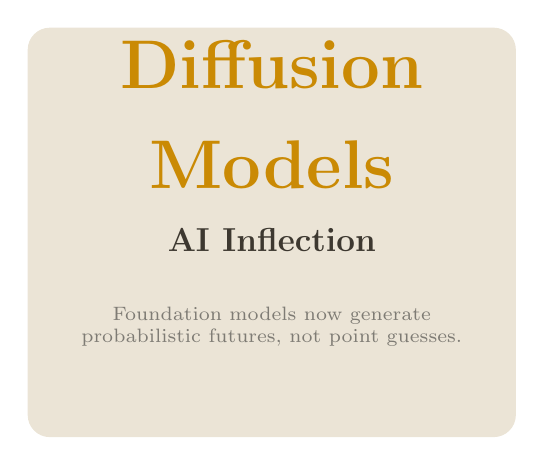
\begin{tikzpicture}
  \fill[hcCard, rounded corners=8pt] (0,0) rectangle (6.2,5.2);
  \node[font=\fontsize{30}{36}\selectfont\bfseries, text=hcGold, align=center] at (3.1,4.1) {Diffusion\\Models};
  \node[font=\large\bfseries, text=hcText] at (3.1,2.5) {AI Inflection};
  \node[font=\scriptsize, text=hcMuted, align=center] at (3.1,1.4) {Foundation models now generate\\probabilistic futures, not point guesses.};
\end{tikzpicture}
\end{center}
\end{column}
\end{columns}

\vspace{16pt}
\begin{center}
\mutedtext{\large Property-level forecasts exist, but no one has built the consumer layer.}
\end{center}
\end{frame}


% ─── SLIDE 6: Market ─────────────────────────────────────────
\begin{frame}{Market: The \$15B Forecast Layer}
\vspace{12pt}

\begin{center}
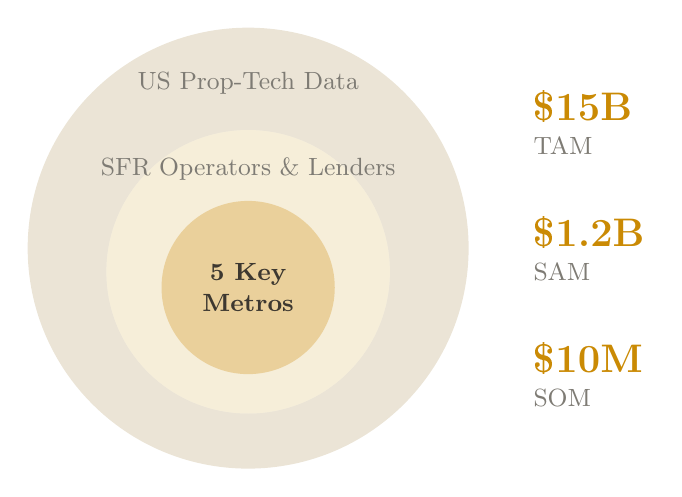
\begin{tikzpicture}
  % TAM
  \fill[hcCard] (0,0) circle (2.8cm);
  \node[text=hcMuted] at (0, 2.1) {\small US Prop-Tech Data};

  % SAM
  \fill[hcBg] (0,-0.3) circle (1.8cm);
  \fill[hcGoldLight!40] (0,-0.3) circle (1.8cm);
  \node[text=hcMuted] at (0, 1.0) {\small SFR Operators \& Lenders};

  % SOM
  \fill[hcGold!40] (0,-0.5) circle (1.1cm);
  \node[text=hcText, font=\small\bfseries, align=center] at (0, -0.5) {5 Key\\Metros};

  % Labels
  \node[text=hcGold, font=\Large\bfseries, anchor=west] at (3.5, 1.8) {\$15B};
  \node[text=hcMuted, font=\small, align=left, anchor=west] at (3.5, 1.3) {TAM};

  \node[text=hcGold, font=\Large\bfseries, anchor=west] at (3.5, 0.2) {\$1.2B};
  \node[text=hcMuted, font=\small, anchor=west] at (3.5, -0.3) {SAM};

  \node[text=hcGold, font=\Large\bfseries, anchor=west] at (3.5, -1.4) {\$10M};
  \node[text=hcMuted, font=\small, anchor=west] at (3.5, -1.9) {SOM};
\end{tikzpicture}
\end{center}

\vspace{4pt}
\begin{center}
\mutedtext{\scriptsize *TAM based on 8M+ investors. SOM reflects Year 3 target in initial metros.}
\end{center}
\end{frame}


% ─── SLIDE 7: Positioning (2x2 Quadrant) ────────────────────
\begin{frame}{Positioning}
\vspace{8pt}

\begin{center}
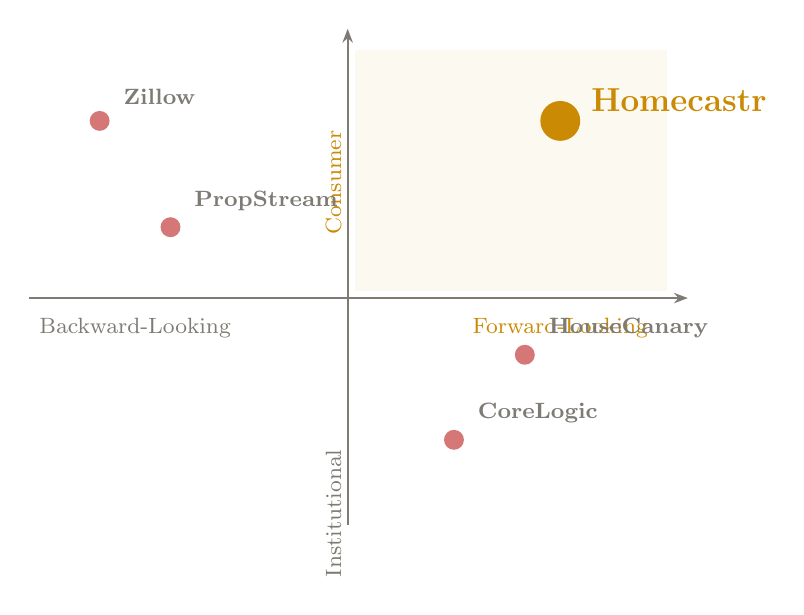
\begin{tikzpicture}[scale=0.9]
  % Axes
  \draw[hcMuted, thick, -{Stealth[length=5pt]}] (-4.5,0) -- (4.8,0);
  \draw[hcMuted, thick, -{Stealth[length=5pt]}] (0,-3.2) -- (0,3.8);

  % Axis labels
  \node[font=\footnotesize, text=hcMuted, anchor=north] at (-3.0,-0.15) {Backward-Looking};
  \node[font=\footnotesize, text=hcGold, anchor=north] at (3.0,-0.15) {Forward-Looking};
  \node[font=\footnotesize, text=hcMuted, anchor=east, rotate=90] at (-0.2,-2.0) {Institutional};
  \node[font=\footnotesize, text=hcGold, anchor=east, rotate=90] at (-0.2,2.5) {Consumer};

  % Quadrant shading — golden quadrant (top-right)
  \fill[hcGoldLight, opacity=0.15] (0.1,0.1) rectangle (4.5,3.5);

  % Competitors — CoreLogic: forward-looking but institutional
  \fill[hcRed!60] (1.5,-2.0) circle (4pt);
  \node[font=\footnotesize\bfseries, text=hcMuted, anchor=south west] at (1.7,-1.9) {CoreLogic};

  % HouseCanary: forward-looking, self-serve, but institutional UX
  \fill[hcRed!60] (2.5,-0.8) circle (4pt);
  \node[font=\footnotesize\bfseries, text=hcMuted, anchor=south west] at (2.7,-0.7) {HouseCanary};

  % PropStream: backward-looking, consumer-ish
  \fill[hcRed!60] (-2.5,1.0) circle (4pt);
  \node[font=\footnotesize\bfseries, text=hcMuted, anchor=south west] at (-2.3,1.1) {PropStream};

  % Zillow: backward-looking, consumer
  \fill[hcRed!60] (-3.5,2.5) circle (4pt);
  \node[font=\footnotesize\bfseries, text=hcMuted, anchor=south west] at (-3.3,2.6) {Zillow};

  % Homecastr — golden quadrant, prominent
  \fill[hcGold] (3.0,2.5) circle (8pt);
  \node[font=\large\bfseries, text=hcGold, anchor=south west] at (3.3,2.5) {Homecastr};

\end{tikzpicture}
\end{center}

\vspace{4pt}
\begin{center}
\goldtext{\textbf{Only consumer-facing, forward-looking platform.}}\\
\mutedtext{\small HouseCanary and CoreLogic forecast forward --- but for analysts, not consumers.}
\end{center}
\end{frame}


% ─── SLIDE 8: Business Model ────────────────────────────────
\begin{frame}{Business Model}
\vspace{12pt}

\begin{columns}[c]
\begin{column}{0.48\textwidth}
\begin{center}
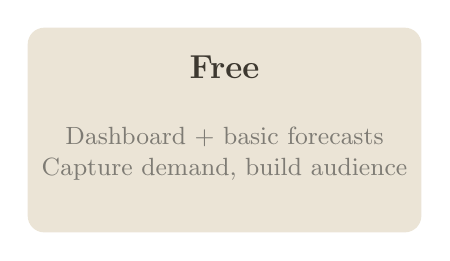
\begin{tikzpicture}
  \fill[hcCard, rounded corners=6pt] (0,0) rectangle (5,2.6);
  \node[font=\large\bfseries, text=hcText] at (2.5,2.1) {Free};
  \node[font=\small, text=hcMuted, align=center] at (2.5,1.0) {Dashboard + basic forecasts\\Capture demand, build audience};
\end{tikzpicture}
\end{center}
\end{column}
\begin{column}{0.04\textwidth}
\begin{center}
{\color{hcGold}\textbf{$\rightarrow$}}
\end{center}
\end{column}
\begin{column}{0.48\textwidth}
\begin{center}
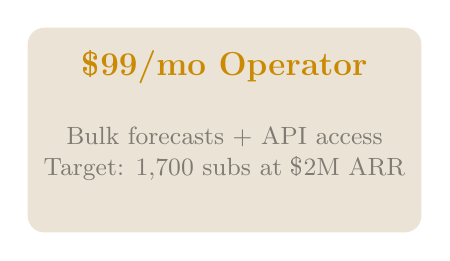
\begin{tikzpicture}
  \fill[hcCard, rounded corners=6pt] (0,0) rectangle (5,2.6);
  \node[font=\large\bfseries, text=hcGold] at (2.5,2.1) {\$99/mo Operator};
  \node[font=\small, text=hcMuted, align=center] at (2.5,1.0) {Bulk forecasts + API access\\Target: 1,700 subs at \$2M ARR};
\end{tikzpicture}
\end{center}
\end{column}
\end{columns}

\vspace{14pt}
\textcolor{hcGoldLight}{\rule{\textwidth}{0.5pt}}
\vspace{8pt}

\begin{center}
\mutedtext{\small Target unit economics: ~\$150 CAC $\cdot$ 24-mo retention $\cdot$ <2 month payback}
\end{center}
\end{frame}


% ─── SLIDE 9: Traction ──────────────────────────────────────
\begin{frame}{Where We Are}
\vspace{20pt}

\begin{center}
\statbox{14\%}{Median Error}
\hfill
\statbox{4yr}{Forecast Horizon}
\hfill
\statbox{Live}{Dashboard}
\hfill
\statbox{Ready}{API}
\end{center}

\vspace{20pt}

\begin{itemize}\setlength{\itemsep}{6pt}
  \item Houston metro: 1M+ properties indexed
  \item Diffusion-based foundation model producing forecast bands
  \item AI voice agent for hands-free exploration
\end{itemize}
\end{frame}


% ─── SLIDE 10: Flywheel ─────────────────────────────────────
\begin{frame}{Flywheel}
\vspace{8pt}

\begin{center}
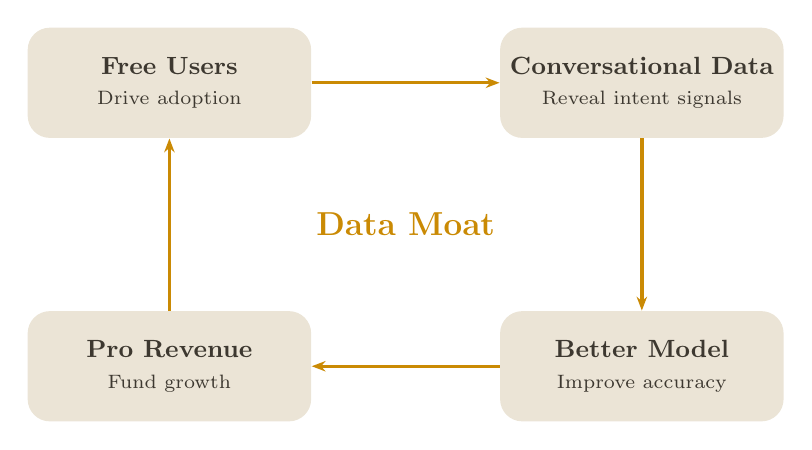
\begin{tikzpicture}[
  block/.style={rounded corners=8pt, fill=hcCard, text=hcText,
    minimum width=3.6cm, minimum height=1.4cm, align=center, font=\small},
  arr/.style={-{Stealth[length=5pt]}, very thick, color=hcGold}
]
  \node[block] (consumers) at (-3.0,1.8) {\textbf{Free Users}\\{\scriptsize Drive adoption}};
  \node[block] (signal) at (3.0,1.8) {\textbf{Conversational Data}\\{\scriptsize Reveal intent signals}};
  \node[block] (model) at (3.0,-1.8) {\textbf{Better Model}\\{\scriptsize Improve accuracy}};
  \node[block] (value) at (-3.0,-1.8) {\textbf{Pro Revenue}\\{\scriptsize Fund growth}};

  \draw[arr] (consumers) -- (signal);
  \draw[arr] (signal) -- (model);
  \draw[arr] (model) -- (value);
  \draw[arr] (value) -- (consumers);

  % Center label
  \node[font=\large\bfseries, text=hcGold] at (0,0) {Data Moat};
\end{tikzpicture}
\end{center}

\vspace{8pt}
\begin{center}
\mutedtext{\small Every query improves the model.\\Every improvement attracts more users.\\Intention data is the long-term asset.}
\end{center}
\end{frame}


% ─── SLIDE 11: Go-to-Market ─────────────────────────────────
\begin{frame}{Go-to-Market}
\vspace{12pt}

\begin{center}
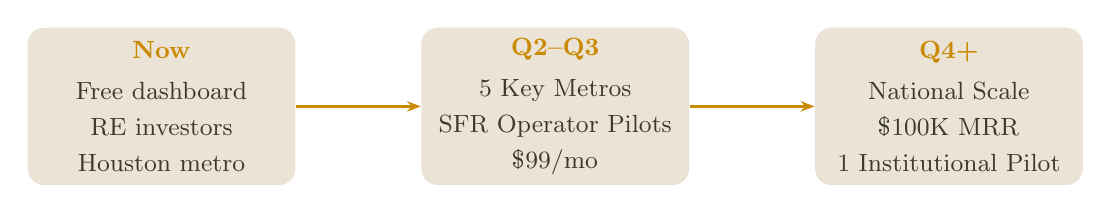
\begin{tikzpicture}[
  phase/.style={rounded corners=6pt, fill=hcCard, text=hcText,
    minimum width=3.4cm, minimum height=2cm, align=center, font=\small},
  arr/.style={-{Stealth[length=5pt]}, thick, color=hcGold}
]
  \node[phase] (p1) at (0,0) {
    \goldtext{\textbf{Now}}\\[4pt]
    Free dashboard\\[2pt]
    RE investors\\[2pt]
    Houston metro
  };
  \node[phase] (p2) at (5,0) {
    \goldtext{\textbf{Q2--Q3}}\\[4pt]
    5 Key Metros\\[2pt]
    SFR Operator Pilots\\[2pt]
     \$99/mo
  };
  \node[phase] (p3) at (10,0) {
    \goldtext{\textbf{Q4+}}\\[4pt]
    National Scale\\[2pt]
    \$100K MRR\\[2pt]
    1 Institutional Pilot
  };

  \draw[arr] (p1) -- (p2);
  \draw[arr] (p2) -- (p3);
\end{tikzpicture}
\end{center}

\vspace{12pt}
\begin{center}
\begin{itemize}\setlength{\itemsep}{8pt}
  \item \goldtext{\textbf{Programmatic SEO}}\\\mutedtext{Capture ``Will [Address] appreciate?'' searches}
  \item \goldtext{\textbf{Broker-Client Loops}}\\\mutedtext{Agents share forecasts with leads}
  \item \goldtext{\textbf{Organic Virality}}\\\mutedtext{Free tool drives word-of-mouth}
\end{itemize}
\end{center}
\end{frame}


% ─── SLIDE 12: Team ──────────────────────────────────────────
\begin{frame}[plain]{Team}
\vspace{4pt}

\begin{columns}[c]
\begin{column}{0.25\textwidth}
\centering
\begin{tikzpicture}
  \node[circle, inner sep=0pt, minimum size=2.5cm, path picture={
    \node at (path picture bounding box.center) {\includegraphics[width=2.5cm]{dhl.jpg}};
  }] {};
\end{tikzpicture}
\end{column}
\begin{column}{0.70\textwidth}
{\Large\bfseries\color{hcGold} Daniel Hardesty Lewis}\\[4pt]
{\large Founder \& CEO}\\[2pt]
\mutedtext{\small \href{https://linkedin.com/in/dhardestylewis}{linkedin.com/in/dhardestylewis}}
\end{column}
\end{columns}

\vspace{8pt}

\begin{columns}[T]
\begin{column}{\textwidth}
\begin{itemize}\setlength{\itemsep}{3pt}
  \item \textbf{Founder, Summit Geospatial}\\\mutedtext{Highest quality terrain in Texas}
  \item \textbf{Sr. Data Scientist, TACC}\\\mutedtext{Principal on \$40M resiliency project}
  \item \textbf{Scientific ML}\\\mutedtext{Bagnold Medal Research Contributor}
  \item \textbf{Teaching}\\\mutedtext{ML for Petrobras Geoscientists}
\end{itemize}
\end{column}
\end{columns}
\end{frame}


% ─── SLIDE 13: The Ask ──────────────────────────────────────
\begin{frame}[c]
\vspace{4pt}

\begin{center}
{\fontsize{36}{42}\selectfont\bfseries\color{hcGold} Raising \$1M}\\[8pt]
{\large Pre-Seed}
\end{center}

\vspace{10pt}

\begin{columns}[T]
\begin{column}{0.49\textwidth}
\textbf{Every Dollar Mapped}\\[6pt]
\begin{itemize}\setlength{\itemsep}{6pt}
  \item \textbf{ML Engineer}\\\mutedtext{Transfer learning to 5 new metros}
  \item \textbf{GTM / Sales}\\\mutedtext{Scale to 1,700+ Operator subs}
  \item \textbf{Data \& Compute}\\\mutedtext{CoreLogic license + GPU training}
\end{itemize}
\end{column}
\begin{column}{0.48\textwidth}
\textbf{18-Month Milestones}\\[6pt]
\begin{itemize}\setlength{\itemsep}{6pt}
  \item \goldtext{\textbf{5 metros}}, 8M+ properties
  \item \goldtext{\textbf{\$50K MRR}} from Operator tier
  \item \goldtext{\textbf{1 institutional pilot}} or LOI
\end{itemize}
\vspace{8pt}
\mutedtext{\scriptsize These milestones position us for Series~A.}
\end{column}
\end{columns}

\vspace{4pt}
\begin{center}
\href{https://homecastr.com}{\goldtext{homecastr.com}} \quad|\quad \href{mailto:daniel@homecastr.com}{\mutedtext{daniel@homecastr.com}}
\end{center}
\end{frame}


% ─── SLIDE 14: Closing Title (Mirror of Slide 1) ────────────
\usebackgroundtemplate{\includegraphics[width=\paperwidth,height=\paperheight]{title_bg.png}}
\begin{frame}[plain]
\vfill
\begin{center}
{\buildingicon}\quad{\fontsize{42}{48}\selectfont\bfseries\color{hcGold} Homecastr}\\[16pt]
{\Large\color{hcText} The foundation model for residential real estate}\\[24pt]
\mutedtext{\small \href{https://homecastr.com}{\textcolor{hcGold}{\textbf{homecastr.com}}}}
\end{center}
\vfill
\end{frame}

\end{document}
